\begin{figure}[htbp]
\centering
\begin{tikzpicture}[x=1cm,y=1cm]
\node[anchor=south west,inner sep=0] at (0,0) {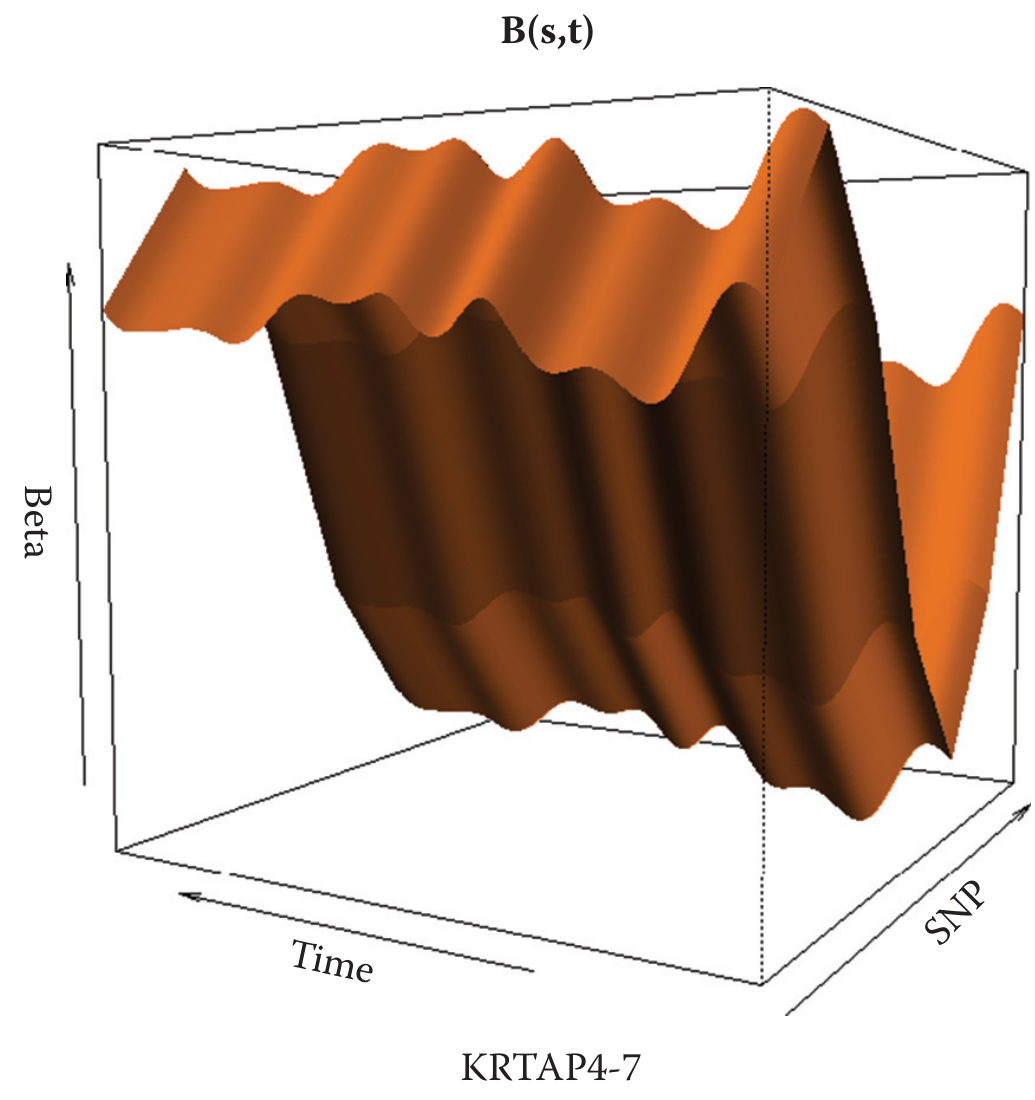
\includegraphics[width=12.0cm]{figures/ch03_fig22_data.png}};
\fill[white] (3.2646,1.2119) rectangle (4.4142,1.9346);
\node[font=\small,rotate=-12,inner sep=0] at (3.8394,1.5732) {时间};
\fill[white] (0.1442,6.2389) rectangle (0.6775,7.1669);
\node[font=\small,rotate=-90,inner sep=0] at (0.4108,6.7029) {$\beta$};
\end{tikzpicture}
\origfig{22}{基因 KPTAP4-7 的遗传效应函数。}
\label{fig:ch03-22}
\end{figure}
